\documentclass[10pt, reqno]{article}
\usepackage{amsmath}
\usepackage{amsfonts}
\usepackage{amssymb}
\usepackage{amsthm}
%american mathematical society - AMS 

\usepackage{hyperref}
\usepackage{float}
\usepackage{enumerate}
\usepackage{graphicx}
\usepackage{wrapfig}
\usepackage{subfig}

\oddsidemargin = 0in
\textwidth=6.5in

\numberwithin{equation}{section} 

\numberwithin{figure}{section}

\title{Calculating Volume from an Implicit Function }
\author{Johnny Minor}
\date{\today}

\begin{document}

\maketitle

\section{Introduction}
In everyday life we may never notice the intricacies of something so simple as a volume. When at the grocery store we can pick up a can of soup and be greeted immediately with the volume of the can in our hand. However, a clever mathematician or engineer had to calculate the volume to make our life easier. Otherwise one might find many seasoned professors looking contemplative in isle seven at Safeway as their mind churns the numbers to find the volume of the can of soup. In this particular paper we will concern ourselves with describing the method of finding the volume of an egg shaped wine fermentation tank. 



\section{Background}
\label{sec:background}

The particular tank that we are interested in calculating the volume of is a tank manufactured by the Sonoma Stone company. 
According to their website the tank has a volume of 476 gallons. \cite{ref:sonoma}

This value is very helpful to guide us as we calculate the volume. It's generally good practice to have a reference value or expression when doing computations. So you're not just blindly clutching at straws. Really it's nice because often times when programming numerical methods you're first attempt probably isn't correct. Without a value to compare to it's very difficult to decipher if you're program is working correctly. 

The equation which describes a cross section of the tank is given to be 
\begin{equation}
0.0002017404542x^2 + \frac{0.0001303290910y}{20.9520444748+\alpha y} = 1.
\end{equation}

\noindent Where $x$ and $y$ are their usual $x$ and $y$ coordinates(measure in centimeters) and $\alpha$ is a constant that changes the overall roundness of the cross section. A lower value of $\alpha$ corresponds to a rounder cross section. A high value corresponds to a less circular cross section, or a more "smushed" shape. For our example the $\alpha$ is equal to $0.005$. 

A natural progression would be to wonder what this unfamiliar equation looks like when plotted. It can be seen that it looks very similar to an egg. %TODO: include cross section of function HERE!!! 

\begin{figure}[H] % 'h' means put it here and 'ht' means that put it at top the and here. 'ht!' put it here now! 
\centering
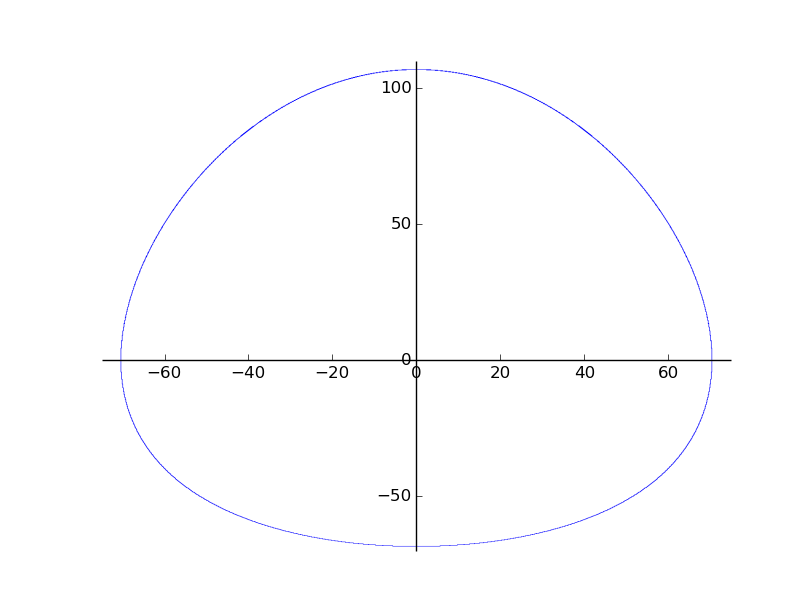
\includegraphics[width=0.5\textwidth]{cross_section.png}
\caption{What a cross section of our function looks like.}
%\label{fig:cross-seciton}
\end{figure}

\noindent And this egg shaped equation spun around the $y$ axis what we hope to solve for. 


\section{Mathematical Method}

It seems like an insurmountable task to a compute a volume integral at first glance of this function. And it would be quite a formidable task without a little help from our friends in form of numpy and scipy. Well, as Professor Cooper says frequently: "We're mathematicians, we know how to do this(paraphrased)." Let's get on it with it then. 

As we learned in our calculus courses. We can use the disc method to integrate our function. The general form of the disc method is to form a shape that resembles a circle. Since we know the area of a circle to be $\pi R^2$ where $R$ is the radius of the circle. If we form an infinite number of discs this will become an integral. This integral will take the form 
\begin{equation}
\label{eq:formula}
\mathrm{Volume}=\pi\int_a^b [R(y)]^2\ \mathrm{d}y. 
\end{equation}

\noindent Where $R(y)$ is our function and $a$ and $b$ are our limits of integration. Although we run into a problem quickly. the equation \ref{eq:formula} is an implicit function. So we first need to solve for $x$ as a function of $y$. This can be done easily with Sympy, but it is an important step in the process nevertheless. 

It is often nice to have a visualization of what's going on. A visual representation of the disc method is like this 

\begin{figure}[H] % 'h' means put it here and 'ht' means that put it at top the and here. 'ht!' put it here now! 
\centering
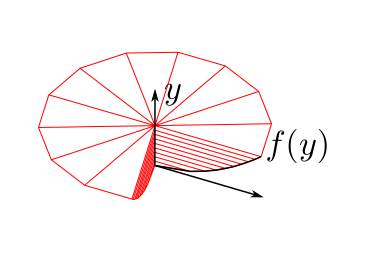
\includegraphics[width=0.4\textwidth]{Disc_integration.png}
\caption{What a cross section integration looks like.\cite{ref:cross_section}}
\label{fig:cross-seciton}
\end{figure}

In figure \ref*{fig:cross-seciton} the function is being rotated around the $y$ axis. 
Now, once the function is solved for $x$ as a function of $y$ then we can use Sympy to carry out the integration for us. This is an easy task for the computer and yields the volume that we're interested in. 

\section{Conclusion}
Using Sympy and Numpy we were easily able to calculate the volume of the egg shaped barrel to be 475.82 gallons which is slightly less than the advertised 476 gallons. In this volume we would expect 2401.59027585 bottles that are 750mL. This isn't a perfectly even value of bottles of wine, but I would speculate there is some quality control testing that takes place before the barrel is bottled for consumption. 

Further in our analysis we varied the value of $\alpha$ and then calculated the corresponding volume of the tank with the given cross section equation. 

\begin{figure}[H] % 'h' means put it here and 'ht' means that put it at top the and here. 'ht!' put it here now! 
\centering
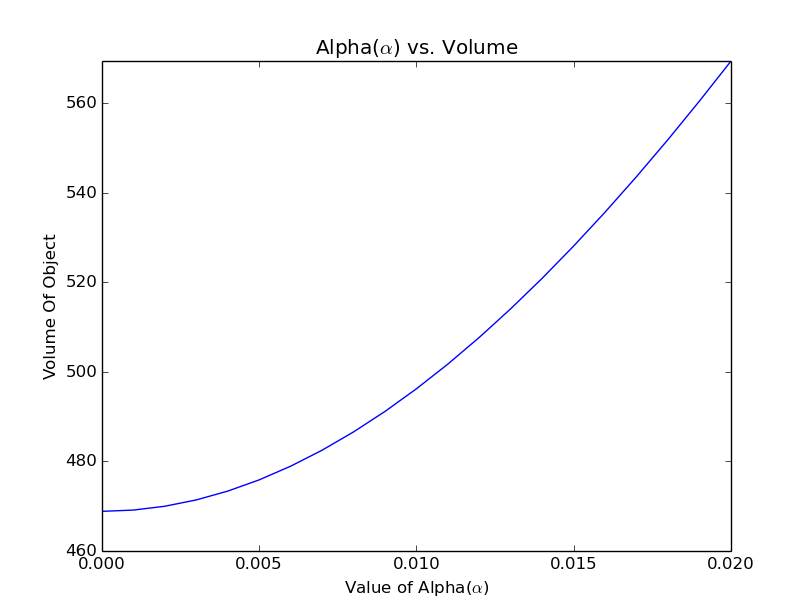
\includegraphics[width=0.8\textwidth]{alpha_volume_plot.png}
\caption{Varying $\alpha$ and calculating the volume}
\label{fig:alpha_volume}
\end{figure}

This is an interesting plot, and it behooves us to do a simple analysis. Figure \ref{fig:alpha_volume} shows that there are actually values of $\alpha$ that would yield a greater volume--interesting. The engineering intentions come to the surface and we might speculate that the egg shape was chosen to minimize floor space while maximizing volume. Perhaps this shape was chosen to help aid in the fermentation process as well. 

Speculation aside, it is an extraordinary feat of mathematics to be able to carry out a calculation via a computer that even the most clever mathematician could only hope to be able to do a mere 400 years ago. 



\begin{thebibliography}{XX}
%TODO: actually fill out the biography. 

\bibitem{ref:cross_section} %when we refer to it by name we use this name. 
Petteri Aimonen (\url{https://en.wikipedia.org/wiki/File:Disc_integration.svg})[Public Domain], via Wikimedia Commons

\bibitem{ref:sonoma} %when we refer to it by name we use this name. 
Sonoma Cast Stone (\url{http://www.concretewinetanks.com/concrete-egg-tank.html}) \today

\end{thebibliography} 




\end{document}